\chapter{Пространственно-временная интерпретация формулы д'Аламбера. Решение
задачи для полубесконечной струны.}

Дадим интерпретацию формулы д'Аламбера для двух частных случаев.
\begin{enumerate}
    \item Начальные условия имеют вид
    \[
        \left\{ \begin{array}{l}
            u(x, 0) = f(x), \\
            \ds \pder{u}{t}(x, 0) = 0.
        \end{array} \right.
    \]
    
    Тогда по формуле д'Аламбера получаем:
    \[
        u(x, t) = \frac{1}{2}\bigl(f(x - ct) + f(x + ct)\bigr).
    \]
    
    Решение \( u \) в точке \( (x_0, t_0) \) можно интерпретировать как среднее
    значение смещений \( f(x) \) в точках \( (x_0 - ct_0, 0) \) и
    \( (x_0 + ct_0, 0) \). Эти точки являются точками пересечения прямых
    \[
        x - ct = x_0 - ct_0, \quad x + ct = x_0 + ct_0
    \]
    с осью \( x \) (рис. \ref{pic19_01}). Указанные прямые называются характеристиками волнового
    уравнения.

    \begin{figure}[h!]
        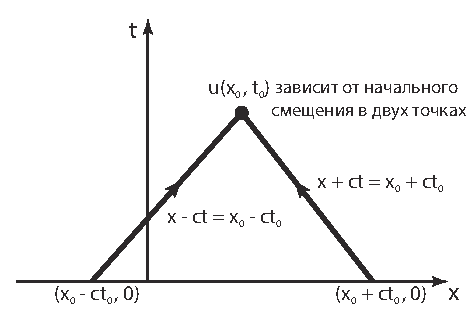
\includegraphics[width=.47\textwidth]{19_01}\hfill
        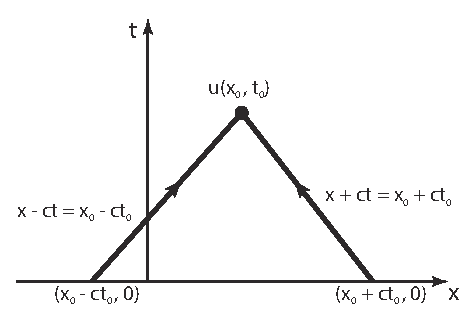
\includegraphics[width=.47\textwidth]{19_03}
        \parbox{.47\textwidth}{\caption{Интерпретация решения с начальным
        смещением без начальной скорости в \( xt \)-плоскости} \label{pic19_01}}
        \hfill
        \parbox{.47\textwidth}{\caption{Интерпретация решения с начальной
        скоростью в \( xt \)-плоскости} \label{pic19_03}}
    \end{figure}

    \item Начальные условия имеют вид
    \[
        \left\{ \begin{array}{l}
            u(x, 0) = 0, \\
            \ds \pder{u}{t}(x, 0) = g(x).
        \end{array} \right.
    \]
    
    Тогда по формуле д'Аламбера получаем:
    \[
        u(x, t) = \frac{1}{2c}\int\limits_{x - ct}^{x + ct} g(\xi)\d\xi.
    \]
    
    Значение величины \( u \) в точке \( (x_0, t_0) \) можно интерпретировать
    как интеграл от начальной скорости в пределах от \( x_0 - ct_0 \) до
    \( x_0 + ct_0 \) (рис. \ref{pic19_03}).
\end{enumerate}

\section{Решение задачи для полубесконечной струны}
\begin{align*}
    & \ppder{u}{t} = c^2\ppder{u}{x}, \quad x \ge 0, \\
    & u(0, t) = 0, \\
    & \left\{ \begin{array}{l}
        u(x, 0) = \phi(x), \\
        \ds \pder{u}{t}(x, 0) = \psi(x).
    \end{array} \right.
\end{align*}

Применяя формулу д'Аламбера, получаем:
\[
    u(x, t) = \frac{1}{2}\bigl(\phi(x - ct) + \phi(x + ct)\bigr) +
    \frac{1}{2c}\int\limits_{x - ct}^{x + ct} \psi(\xi)\d\xi.
\]

Однако, функции \( \phi \) и \( \psi \) определены лишь для положительного
аргумента. Так как \( x - ct \) может принимать и отрицательные значения, то
требуется доопределить \( \phi \) и \( \psi \) на отрицательной полуоси.
Воспользуемся граничным условием:
\[
    u(0, t) = 0 \Rightarrow \frac{1}{2}\bigl(\phi(-ct) + \phi(ct)\bigr) +
    \frac{1}{2c}\int\limits_{-ct}^{ct} \psi(\xi)\d\xi = 0.
\]

В силу независимости функций \( \phi \) и \( \psi \) равенство возможно лишь при
\( \phi(-ct) = \phi(ct) \) и \( \psi(-ct) = -\psi(ct) \). Таким образом, в
случае \( x - ct < 0 \) имеет место решение:
\[
    u(x, t) = \frac{1}{2}\bigl(\phi(x + ct) - \phi(ct - x)\bigr) +
    \frac{1}{2c}\int\limits_{ct - x}^{x + ct} \psi(\xi)\d\xi.
\]

Комбинируя решения, окончательно получим:
\[
    u(x, t) = \frac{1}{2}\bigl(\phi(x + ct) - \phi(|x - ct|)\bigr) +
    \frac{1}{2c}\int\limits_{|x - ct|}^{x + ct} \psi(\xi)\d\xi.
\]
\newpage
